\PassOptionsToPackage{dvipdfmx}{graphicx}% NOTE: only for Japanese
\PassOptionsToPackage{dvipdfmx}{xcolor}% NOTE: only for Japanese
\documentclass[sip,biber]{now-journal}
\addbibresource{ref.bib}

\usepackage[nolist,nohyperlinks]{acronym}
\usepackage{amsfonts}
\usepackage{bm}
\usepackage{mathtools}
\usepackage{siunitx}
\usepackage{subcaption}

% reload hyperref
\usepackage[colorlinks=true, allcolors=blue, plainpages=false, pdfpagelabels=true]{hyperref}
\usepackage{breakurl}

% cleveref setting
\usepackage[capitalise]{cleveref}
\crefformat{equation}{(#2#1#3)}
\Crefformat{equation}{#2Equation~(#1)#3}
\crefformat{section}{Section~#2#1{}#3}
\crefname{algorithm}{Algorithm}{Algorithms}
\crefname{equation}{}{}
\crefname{figure}{Figure}{Figures}
\crefname{section}{Section}{Sections}
\def\crefrangeconjunction{--}

% psuedo codes
\usepackage{xcolor}
\usepackage[theorems,skins]{tcolorbox}
\usepackage{tabularx}
\usepackage{pseudo}
\newtcbtheorem[crefname = {Algorithm}{algorithms}]{algorithm}{Algorithm}{pseudo/booktabs, float=t, theorem hanging indent=0pt}{alg}
\pseudodefinestyle{fullwidth}{
    begin-tabular=
    \tabularx{\textwidth}[t]{@{}
        r                                          % Labels
        >{\leavevmode\pseudosetup}                 % Indent, font, ...
        X                                          % Code (flexible)
        >{\leavevmode} % Comment styling
        p{0.20\textwidth}                           % Comments (fixed)
        @{}},
    end-tabular=\endtabularx,
}
\pseudoset{%
   fullwidth,
   kwfont=\sffamily\bfseries,
   font=\kwfont,
   prfont=\textsf,
   hsep=.3em,
   indent-mark,
   indent-mark-shift=.5em,
   indent-length=1em,
   line-height=1.5,
   ct-left=\hfill\texttt{//}~,
   ct-right=,
   % label=\textcircled{\ttfamily\scriptsize\arabic*},
   label=,
   % ref,
}

% Align euqality or replacement in pseudo codes
% ref: https://latex.org/forum/viewtopic.php?t=26363
\usepackage{xparse}
\DeclareDocumentCommand{\psm}{m O{$\gets$}}{% pseudocode-math
  {\hphantom{$W_{k,f,t - 1}$}\llap{#1}~#2}%
  % {\rlap{#1}\hphantom{$W_{k,f,t}$}#2}%
}

% Original style files
\usepackage{bsssym}

% Document information
\title{Self-Rotation-Robust Online Independent Vector Analysis with\\Sound Field Interpolation on Circular Microphone Array}
\fancyhead[LO]{\footnotesize\textit{Self-rotation-robust online independent vector analysis with sound field interpolation on circular microphone array}}
\author{Nakashima, Taishi}
\affil{Tokyo Metropolitan University, Tokyo, Japan}
\author{Wakabayashi, Yukoh}
\affil{Toyohashi University of Technology, Aichi, Japan}
\author[1]{Ono, Nobutaka}
\creditline{%
  Corresponding author: Taishi Nakashima, \href{mailto:taishi@ieee.org}{taishi@ieee.org}.
  This work was supported by JSPS KAKENHI Grant Number 21J22039 and JST CREST Grant Number JPMJCR19A3.
}

\articledatabox{
  Received XX June 2023; Revised YY Sep 2023
  ISSN XXXX-YYYY; DOI xx.yyyy/zzz.wwwwwwww\\
  \copyright 2023 T. Nakashima, Y. Wakabayashi, and N. Ono
}

\keywords{
  Blind source separation,
  online independent vector analysis,
  circular microphone array,
  sound field interpolation
}

\begin{document}

\begin{abstract}
  % 本論文では,マイクロホンアレイの回転に頑健なオンラインブラインド音源分離手法を提案する.
  % Online auxiliary-function-based independent vector analysis (OIVA)はリアルタイムBSSを実現するための有望な手法のひとつである.
  % リアルタイムBSSを実用化するためには,音源やマイクの移動といった環境の変化に対する頑健性が重要な課題である.
  % 一般的にリアルタイム処理の最中に環境の変化が起こった場合はパラメータの再推定が必要である.
  % OIVAでは音源のなめらかな移動に対して頑健かつ高い分離性能を獲得できることが示されていた.
  % しかし,OIVAはマイクの突発的な移動に対しては十分な性能が得られない.
  % そこで本論文では,円状等間隔マイクロホンアレイ(CMA)のための音場補間処理を利用したOIVAを提案する.
  % 音場補間はCMAの回転を打ち消し,パラメータの再推定を必要とせずにBSSを可能にする.
  % シミュレーション実験の結果は音場補間によりマイクが回転する状況における音源分離の頑健性が向上したことを確認した.
  In this paper, we propose robust online blind source separation (BSS) method against self-rotation of microphone arrays.
  Online auxiliary-function-based independent vector analysis (OIVA) is one of the promising methods for real-time BSS.
  One major issue for real-time BSS is robustness against environmental changes such as movement of source or microphone.
  In general, parameter re-estimation is necessary if environmental changes occur during real-time processing.
  OIVA has been shown to be robust against smooth movement of sources and to achieve high separation performance.
  However, OIVA does not perform well against sudden movements of microphones.
  Therefore, in this paper, we employ the sound field interpolation (SFI) for circular microphone arrays (CMAs) with OIVA.
  SFI cancels out rotation of the CMA, enabling us to apply BSS without parameter re-estimation.
  Simulation experiments confirmed that SFI improves the robustness of the OIVA in situations where the microphone is rotating.
\end{abstract}

\section{Introduction}
% ブラインド音源分離など多くのアレイ信号処理では,時不変な系を仮定する.
% しかし,実応用のためにはマイクロホンや音源の移動など系の時間変化を考慮する必要がある.
% そこで,系の時間変化のひとつとして,円状等間隔マイクロホンアレイ(circular microphone array; CMA)の回転を考え,音場の補間により対応する手法 \cite{Wakabayashi:2020:ASJ:A} が提案された.
% この手法はCMAの対称性を利用することで,CMAが回転する前の音場を簡単な線形演算により推定する.
% また,ビームフォーミング \cite{Wakabayashi:2021:ICASSP} やステアリングベクトル推定 \cite{Wakabayashi:2021:ASJ:A} への応用や,
% CMAの回転角度を自己推定する手法 \cite{Lian:2021:APSIPA} も提案されている.
% 本稿では,CMAが回転する状況下のブラインド音源分離に取り組む.
% 音場補間によりCMAの回転の影響を打ち消し,後段にブラインド音源分離を適用する.
% さらに,シミュレーション実験により音源分離性能を評価する.
Most array signal processing methods, such as blind source separation (BSS), assume a time-invariant system.
However, for practical applications, it is necessary to consider time variations of the system, such as movements of the microphone or source.
Sound field interpolation for circular microphone array (CMA) \cite{Wakabayashi:2021:ICASSP} has been proposed to address the rotation of a CMA as one of the time variations of the system.
This method exploits the symmetry of the CMA to estimate the sound field before the rotation of the CMA by a simple linear operation.
Applications to beamforming \cite{Wakabayashi:2021:ICASSP} and steering vector estimation \cite{Wakabayashi:2021:ASJ:A} have also been proposed,
as well as a method for self-estimating the rotation angle of a CMA \cite{Lian:2021:APSIPA}.
In this paper, we address blind source separation in situations where the CMA rotates.
The effect of the rotational movement of the CMA is counteracted by interpolating the sound field, and blind source separation is applied in the latter stage.
Furthermore, the source separation performance is evaluated by simulation experiments.

\section{Problem Formulation}
% 回転するかもしれない,円状アレイ前提なのでセンサーの数・配置など明記
\begin{table}[t]
  \centering
  \caption{Symbols}
  \begin{tabular}{ll}
    \toprule
      Symbol & Description \\
    \midrule
      $\Mic$                                                     & Number of microphones \\
      $\Src$                                                     & Number of sources \\
      $\steer _{\src,\ft} \in \C ^{\Mic}$                        & Steering vector \\
      $\sig _{\src,\ft} \in \C$                                  & Source signal \\
      $\Obs _{\ft} \in \C^{\Mic}$                                & Observed signal at \textcolor{red}{\textbf{initial position}} \\
      $\rotDeg \in \R$                                           & Rotation angle \\
      $\rotFra \in \R$                                           & Rotation time \\
      $\rotMat _{\rotDeg} \in \R ^{\Mic \times \Mic}$            & Rotation matrix \\
      $\rotObs _{\ft} \coloneqq \rotMat _{\rotDeg} \Obs _{\ft}$  & Observes signal after \textcolor{red}{\textbf{rotation}} \\
      $\Demix _{\ft}$                                            & Demixing matrix \\
      $\Est _{\ft} \coloneqq \Demix _{\ft} \Obs _{\ft}$          & Estimated signal \\
      $\cov _{\src,\ft}$                                         & Covariance matrix \\
    \bottomrule
  \end{tabular}
\end{table}

Let $\Src$ and $\Mic$ respectively be the number of sources and microphones.
We assume that the observed signal $\Obs _{\ft}$ is modelled as:
\begin{equation}
  \Obs _{\ft} = \sum _{\src=1} ^{\Src} \steer _{\src\ft} \sig _{\src\ft},
\end{equation}
in the short-time Fourier transform (STFT) domain,
where $\freq = 1, \dots, \Freq$ denotes the frequency bin index,
$\tframe = 1, \dots, \Tframe$ denotes the time frame index,
$\sig _{\src\ft} \in \C\; (\src = 1, \dots, \Src)$ denotes the $\src$-th source signal, and
$\steer _{\src\ft} \in \C ^{\Mic}\; (\src = 1, \dots, \Mic)$ denotes the steering vector of $\src$th source signal to each microphone.

% オンラインブラインド音源分離の目的は,現在と過去の観測信号$\{\obs _{\freq,i}\} _{i=1} ^{\tframe}$のみを用いて,
% 分離行列を推定し,音源を分離することである:
% \begin{align}
%   \Demix _{\ft} &= \begin{bmatrix} \demix _{1\ft} & \dots & \demix _{\Src\ft} \end{bmatrix} ^{\hermite} \in \C ^{\Src \times \Mic}, \\
%   \est _{\ft} &= \Demix _{\ft} \obs _{\ft} \in \C ^{\Src},
% \end{align}
% ここで,$\Demix _{\ft}$は分離行列,$\est _{\ft}$は分離信号である.
% 本研究では,ある時間フレーム$\rotFra$においてCMAが角度$\rotDeg$回転した状況下で分離行列を推定することを考える.
% ただし,$\rotFra$および$\rotDeg$は既知とする.
Online blind source separation aims to estimate the demixing matrix and estimated signals using only the current and past observed signals $\{\Obs _{\freq,i}\} _{i=1} ^{\tframe}$:
\begin{align}
  \Demix _{\ft} &= \begin{bmatrix} \demix _{1\ft} & \dots & \demix _{\Src\ft} \end{bmatrix} ^{\hermite} \in \C ^{\Src \times \Mic}, \\
  \Est _{\ft} &= \Demix _{\ft} \Obs _{\ft} \in \C ^{\Src},
\end{align}
where $\Demix _{\ft}$ is the demixing matrix and $\Est _{\ft}$ is the estimated signal.
We consider estimating the demixing matrix in a situation where the CMA is rotated by an angle $\rotDeg$ in a certain time frame $\rotFra$.
Please note that $\rotFra$ and $\rotDeg$ are assumed to be known in this study.% because we focus only on the efficacy of sound field interpolation.

\section{Proposed method}

CMAが回転した後の位置における観測信号$\rotObs _{\ft}\; (\tframe \geq \rotFra)$と,ある行列$\rotMat (\rotDeg) \in \R ^{\Mic\times\Mic}$を用いて,
CMAが回転する前の位置における観測信号$\Obs _{\ft}$を推定することを考える.
\begin{equation}
  \rot{\Obs} _{\ft} = \rotMat (\rotDeg) \Obs _{\ft},
\end{equation}
$\rotMat (\rotDeg)$の計算方法の詳細は文献 \cite{Wakabayashi:2020:ASJ:A} を見よ.
$\rotMat (\rotDeg)$が推定できれば,CMAが回転する前の位置における観測信号は$\Obs _{\ft} = \rotMat (-\rotDeg) \rot{\Obs} _{\ft}$と表せる.
CMAが回転する前の時間フレーム$\tframe < \rotFra$における観測信号$\Obs _{\ft}$を用いて分離行列$\Demix _{\ft}$が推定できていたとする.
音場補間を適用し,回転前の観測信号を推定することで,CMAが回転した後も分離行列を推定し直すことなく分離信号$\Est _{\ft}$が得られる.
\begin{equation}
  \Est _{\ft} = \Demix _{\ft} \rotObs _{\ft} = \Demix _{\ft} \left(\rotMat (\rotDeg)^{-1} \Obs _{\ft}\right).
\end{equation}

本論文では,補助関数型独立ベクトル分析 (auxiliary-function-based independent vector analysis; AuxIVA) \cite{Ono:2011:WASPAA}
およびそのオンライン拡張 (online AuxIVA; OIVA) \cite{Taniguchi:2014:HSCMA} を用いて音源分離を行う.
AuxIVAでは,各音源$\src = 1, \dots, \Src$に対して次の更新式で時不変な分離行列$\Demix _{\freq}$を推定する.
\begin{align}
  \var _{\src\tframe} &\gets \sqrt{\sum _{\freq=1} ^{\Freq} \lvert \demix ^{\hermite} _{\src\freq} \Obs ^{\nohermite}_{\ft} \rvert ^2}, \\
  \cov _{\src\freq} &\gets \frac{1}{\Tframe} \sum _{\tframe=1} ^{\Tframe} \weight (\var_{\src\tframe}) \Obs _{\ft} \Obs _{\ft}^{\hermite}, \\
  \demix _{\src\freq} &\gets (\Demix _{\freq} \cov _{\src\freq}) ^{-1} \eye _{\src} \label{eq:ip:proj}, \\
  \demix _{\src\freq} &\gets {\demix _{\src\freq}} / {\sqrt{\demix _{\src\freq} ^{\hermite} \cov _{\src\freq} \demix _{\src\freq}}} \label{eq:ip:norm}.
\end{align}
ここで,$\eye _{\src}$は単位行列の$\src$列目のベクトルである.
$\cov _{\src\freq}$は{重み付き共分散行列}と呼ばれる.
$\weight(\var)$は音源モデルによって定まる関数であり,
本論文では時変Gauss分布を仮定した場合に対応する,$\weight (\var) = \Freq/{\var ^2}$ \cite{Ono:2012:APSIPA}を用いる.

OIVAでは,時間フレーム$\tframe$ごと重み付き共分散行列$\cov _{\src\ft}$を更新する~\cite{Taniguchi:2014:HSCMA}.
\begin{equation}
  \cov _{\src\ft} \gets \forget \cov _{\src\freq(\tframe-1)} + (1 - \forget) \weight ({\var _{\src\tframe}}) \Obs _{\ft} \Obs _{\ft}^{\hermite}.
\end{equation}
ここで,$\forget\; (0 \leq \forget < 1)$は忘却係数である.
分離行列は\cref{eq:ip:proj}, \cref{eq:ip:norm}と同じ更新式を用いて書く時間フレームで更新する.
両方の手法において,CMAの回転を含む観測信号に対して,音場補間を適用した後の信号を改めて入力する.

% It is shown how to approximate x̂=U(θ)x using a certain matrix U (θ) ∈ CM ×M, with the observed signal x̂ (t ≥ t̂) at the position after the microphone has rotated (see [1] for details).
% Suppose that the separation matrix W could be estimated using the observed signal x in time frame t<t̂ before the CMA was rotated.
% By applying sound field interpolation and estimating the observed signal before the rotation as follows, the separation signal y can be obtained after the CMA has rotated without having to re-estimate the separation matrix.

% In this paper, auxiliary-function-based independent vector analysis (AuxIVA) [5] and its online extension (online AuxIVA; OIVA) [6] are used as source separation methods.
% In AuxIVA, each source k = 1, . . . K, the time-invariant separation matrix W is estimated with the following update formula

% where ek is the kth column vector of the identity matrix.
% Vkf is called the weighted covariance matrix.
% φ(r) is a function determined by the source model, and in this paper the time-invariant Gauss distribution φ(r) = F/r2 [7].
% OIVA, on the other hand, updates the weighted covariance matrix Vkf t for each time frame t [6].
% where α (0 ≤ α < 1) is the forgetting factor. The separation matrix is updated in the time frame in which it is written using the same update formula as in eq. (8), eq. (9).
% For both methods, the signal is input again after applying the sound field interpolation to the observed signal including the CMA rotation.

\subsection{Frequency band limitation (\textcolor{red}{\textbf{WiP}})}
\begin{itemize}
  \item 音場補間は周波数が高くなるほどモデルとの乖離が大きくなり補間性能が悪くなる \cite{Wakabayashi:2020:ASJ:A}
  \item 音源分離に用いる音源モデル$\var _{\src\tframe}$を計算するとき,補間がうまくできている周波数帯域だけで計算すれば分離性能が改善されると期待できる
  \item サンプリング周波数$\freqSamp~\unit{\hertz}$,FFT点数$\nfft$のとき,STFTの周波数ビンインデクス$\freq$と物理的な周波数$\freqPhys$の対応
    \begin{equation}
      \freqPhys = \frac{(\freq - 1)\times\freqSamp}{\nfft} \quad \left(\freq = 1, \dots, \frac{\nfft}{2} + 1\right),
    \end{equation}
  \item 修正された音源モデルの更新式
    \begin{equation}
      \var _{\src\tframe} = \sqrt{\sum _{\freq = 1} ^{\SubFreq} \lvert \demix _{\src\ft} \Obs _{\ft} \rvert ^2},
    \end{equation}
    ただし,$\SubFreq$は周波数の上限
\end{itemize}

\subsection{Coordinate transformation of sound field interpolation}
\subsubsection{Purpose}
\begin{itemize}
  \item 究極の目的: マイクの回転に頑健なオンライン音源分離を開発したい
  \item 音源分離では観測信号を ``混ぜ直して'' 新たに入力としても出力は変わらないはず
    \begin{itemize}
      \item ``混ぜ直し''例: 2chの入力$x_1, x_2$を$x_1+x_2, x_1-x_2$と改めて入力
      \item 音場補間も一種の``混ぜ直し''
        \begin{itemize}
          \item 音場補間があってもなくても分離性能は変わらなさそうだが,以前の結果はそうではない
          \item[$\Rightarrow$] わざわざ音場補間を行う意義を明らかにしたい
        \end{itemize}
    \end{itemize}
  \item マイク回転前までに得られた共分散$\cov _{\src,\ft}$を活用したい
    \begin{itemize}
      \item[$\Rightarrow$] 回転時に$\cov _{\src,\ft},\, \Demix _{\ft}$を ``座標変換''
    \end{itemize}
\end{itemize}

\subsubsection{共分散・分離行列の``座標変換''}
\begin{align}
  \rot{\cov} _{\src,\freq} &\coloneqq \frac{1}{\Tframe} \sum _{\tframe = 1} ^{\Tframe} \weight (\var _{\src,\tframe}) \rotObs _{\ft} \rotObs _{\ft} ^{\hermite} \\
                           &= \frac{1}{\Tframe} \sum _{\tframe = 1} ^{\Tframe} \weight (\var _{\src,\tframe}) (\rotMat _{\rotDeg} \Obs _{\ft}) (\Obs _{\ft} ^{\hermite} \rotMat _{\rotDeg} ^{\hermite}) \\
                           &= \rotMat _{\rotDeg} \left(\frac{1}{\Tframe} \sum _{\tframe = 1} ^{\Tframe} \weight (\var _{\src,\tframe}) \Obs _{\ft} \Obs _{\ft} ^{\hermite}\right) \rotMat _{\rotDeg} ^{\hermite} \\
                           &= \rotMat _{\rotDeg} \cov _{\src,\freq} \rotMat _{\rotDeg} ^{\hermite}
  \\
  \Est _{\ft} &= \Demix _{\ft} \Obs _{\ft} \\
              &= \Demix _{\ft} \underbrace{(\rotMat _{\rotDeg} ^{\hermite} \rotMat _{\rotDeg})}_{=I} \Obs _{\ft} \\
              &= \underbrace{(\Demix _{\ft} \rotMat _{\rotDeg} ^{\hermite})}_{\coloneqq \rotDemix _{\ft}} (\rotMat _{\rotDeg} \Obs _{\ft}) \\
              &= \rotDemix _{\ft} \rotObs _{\ft}
\end{align}

\section{実験}
\subsection*{目的}
\begin{itemize}
  \item 座標変換の有効性の確認
  \item 座標変換と通常の音場補間との性能差を確認
\end{itemize}

\subsection*{条件}
\begin{figure}[t]
  \centering
  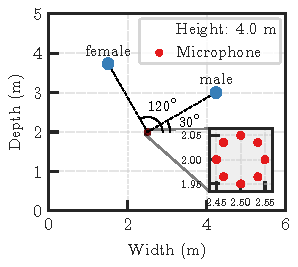
\includegraphics{figures/room_layout.pdf}
  \caption{Room layout.}%
  \label{fig:layout}
\end{figure}
\begin{itemize}
  \item 音源・マイク配置 (\cref{fig:layout}), 5音源5マイク
    % \begin{itemize}
    %   \item 前は2音源5マイクでやっていたが評価がよくわからなくなった…
    %     \begin{itemize}
    %       \item 参考:\href{https://github.com/onolab-tmu/overiva/blob/1cb3189112889ebfe2ccbbde0f55b1db6020fc48/overiva_sim.py#L200}{OverIVAの評価}\\
    %         分離信号の余ったチャネルをrandnで埋める
    %     \end{itemize}
    %   \item 分離音が複数チャネルに分かれる場合の評価方法?
    %   \item 分離されているとも言えるが,望ましい結果とは言えない…
    %   \item[$\Rightarrow$] 簡単のためにいったん決定条件でやり直した
    % \end{itemize}
  \item 残響時間: 約\SI{100}{\milli\second}
  \item マイク間隔: \SI{2}{\centi\metre}
  \item マイク回転角度: \SI{40}{\degree} at \SI{30}{\second}
  \item STFT: FFT長 4096, 1/2-shift, Hamming窓
  \item Projection back: \cref{alg:pb}, 参照マイク=1
  \item SI-SDRの参照信号: 各音源の音像(途中でマイクが回転する)
\end{itemize}

\subsection{結果}
% - 忘却係数 0.99 -> 回転にあまり追従しないようにしておく
\begin{itemize}
  \item 比較手法
    \begin{itemize}
      \item \Cref{alg:naive}: 通常のOnline AuxIVA (\textbf{Naive})
      \item \Cref{alg:reset}: 回転後に$\Demix _{\ft}, \cov _{\src,\ft}$を初期化 (\textbf{Reset})
      \item \Cref{alg:sfi}: 回転後に観測信号の回転を補償 (\textbf{RT-obs})\\
        $\Obs _{\ft} = \rotMat _{\rotDeg} ^{-1} \rotObs _{\ft}$
      \item \Cref{alg:coord}: 回転後に$\Demix _{\ft}, \cov _{\src,\ft}$を``座標変換'' (\textbf{RT-cov})\\
        $\rotDemix _{\ft} \gets \Demix _{\ft} \rotMat _{\rotDeg} ^{\hermite}$,\; $\rotCov _{\src,\ft} \gets \rotMat _{\rotDeg} \cov _{\src,\ft} \rotMat _{\rotDeg} ^{\hermite}$
    % \begin{itemize}
    %   \item $\cov _{\src,\ft[-1]}$はそれ以前のすべての観測の情報を含んでいるので,それだけに$\rotMat _{\rotDeg}$をかけて,あとは観測をそのまま使って更新すればいいはず
    % \end{itemize}
    \end{itemize}
  \item パラメータ
    \begin{itemize}
      \item 初期値: $\Demix _{\freq,0} = \Eye\; (\forall \freq)$, $\cov _{\src,\freq,0} = 10^{-3}\times\Eye\; (\forall \src, \freq)$
      \item 忘却係数$\forget$: 0.90, 0.91, ..., 0.99
      \item 音源モデル: 時変Gauss
      \item フレームごとの反復回数$\Itr$: 5
      \item 正則化: $\cov _{\src,\ft} \gets \cov _{\src,\ft} + 10 ^{-3} \Eye$
    \end{itemize}
\end{itemize}

\begin{figure}[t]
  \begin{minipage}[t]{.5\linewidth}
    \centering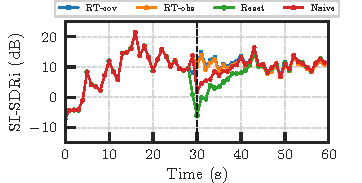
\includegraphics{figures/plots/online/Gauss_8000_fft4096_90.pdf}\subcaption{$\forget = 0.90$}\label{fig:plot:gauss:90}
    \centering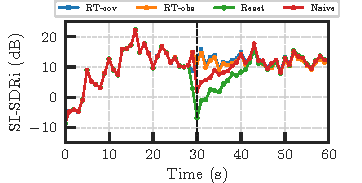
\includegraphics{figures/plots/online/Gauss_8000_fft4096_91.pdf}\subcaption{$\forget = 0.91$}\label{fig:plot:gauss:91}
    \centering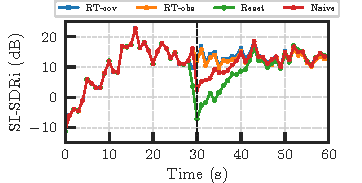
\includegraphics{figures/plots/online/Gauss_8000_fft4096_92.pdf}\subcaption{$\forget = 0.92$}\label{fig:plot:gauss:92}
    \centering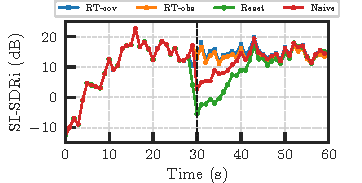
\includegraphics{figures/plots/online/Gauss_8000_fft4096_93.pdf}\subcaption{$\forget = 0.93$}\label{fig:plot:gauss:93}
    \centering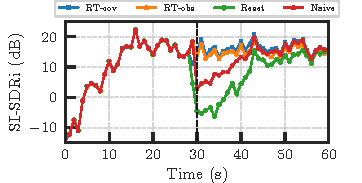
\includegraphics{figures/plots/online/Gauss_8000_fft4096_94.pdf}\subcaption{$\forget = 0.94$}\label{fig:plot:gauss:94}
  \end{minipage}%
  \begin{minipage}[t]{.5\linewidth}
    \centering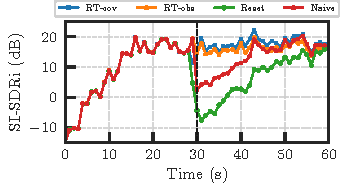
\includegraphics{figures/plots/online/Gauss_8000_fft4096_95.pdf}\subcaption{$\forget = 0.95$}\label{fig:plot:gauss:95}
    \centering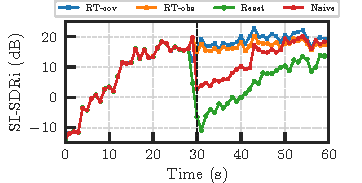
\includegraphics{figures/plots/online/Gauss_8000_fft4096_96.pdf}\subcaption{$\forget = 0.96$}\label{fig:plot:gauss:96}
    \centering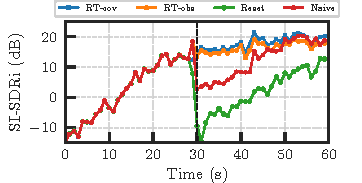
\includegraphics{figures/plots/online/Gauss_8000_fft4096_97.pdf}\subcaption{$\forget = 0.97$}\label{fig:plot:gauss:97}
    \centering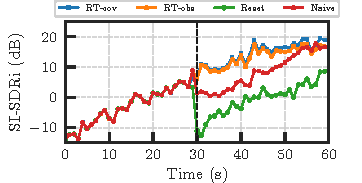
\includegraphics{figures/plots/online/Gauss_8000_fft4096_98.pdf}\subcaption{$\forget = 0.98$}\label{fig:plot:gauss:98}
    \centering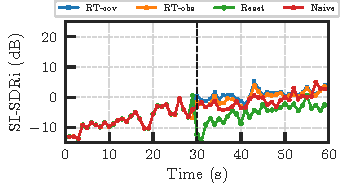
\includegraphics{figures/plots/online/Gauss_8000_fft4096_99.pdf}\subcaption{$\forget = 0.99$}\label{fig:plot:gauss:99}
  \end{minipage}
  \caption{Segmental SI-SDR improvements (SI-SDRi) every \SI{1}{\second} with $\Src = \Mic = 5$ and $\text{RT}_{60} \approx \SI{100}{\milli\second}$.}
\end{figure}

\paragraph{雑感・メモ}
\begin{itemize}
  \item 実験結果
    \begin{itemize}
      \item RT-cov
        \begin{itemize}
          \item マイク回転後も分離性能の低下がほとんどない
        \end{itemize}
      \item RT-obs
        \begin{itemize}
          \item RT-covとほとんど同じ
          \item 最終的な分離性能はRT-covにわずかに劣る
            \begin{itemize}
              \item 音源分離はマイク回転を補償した観測信号,\\性能評価はマイク回転ありの音像を用いているため?
            \end{itemize}
        \end{itemize}
      \item Reset
        \begin{itemize}
          \item 回転後に大きく性能が低下
          \item 回転後は徐々に収束
          \item 忘却係数$\forget$が1に近づくほど回転前後の性能差が大きくなる
        \end{itemize}
      \item Naive
        \begin{itemize}
          \item 回転後に大きく性能が低下,低下の幅はResetよりも小さく,ほとんどすべての忘却係数について同じくらい
        \end{itemize}
    \end{itemize}
  \item その他
    \begin{itemize}
      \item FFT長2048以下,忘却係数0.95以下で$\cov _{\src,\ft} ^{-1}$が発散する
    \end{itemize}
\end{itemize}

\paragraph*{疑問}
\begin{itemize}
  \item オンラインAuxIVAでの共分散行列 ``座標変換'' ?\\ バッチの場合と勝手が違う気がする…\\
    マイクは $\tframe \leq \rotFra - 1$ で基準位置,
    $\tframe \geq \rotFra$ で回転後とする.
    \begin{align*}
      \rot{\cov} _{\src,\ft} &= \forget \cov _{\src,\ft[-1]} + (1 - \forget) \weight(\var _{\src,\tframe}) \rot{\Obs} _{\ft} \rot{\Obs} _{\ft} ^{\hermite} \\
                             &= \forget ^{\tframe} \cov _{\src,\freq,0}
                                + \sum _{i = 1} ^{\rotFra - 1} \forget ^{\tframe - i} (1 - \forget) \weight(\var _{\src,i}) \Obs _{\freq,i} \Obs _{\freq,i} ^{\hermite} \\
                             &\qquad + \sum _{j = \rotFra} ^{\tframe} \forget ^{\tframe - j} (1 - \forget) \weight(\var _{\src,j}) \rot{\Obs} _{\freq,j} \rot{\Obs} _{\freq,j} ^{\hermite}
    \end{align*}
  \item 音場補間,座標変換のいい感じの名前?ロボット工学の用語でワールド座標系,ロボット座標系などがあるが,これをもじって簡潔に言い表せないか?
\end{itemize}

\paragraph*{TODO}
\begin{itemize}
  \item 忘却係数を周波数ごとに設計
    \begin{itemize}
      \item 音場補間は高周波数帯では動かないので高い周波数は早く忘れるようにする?
    \end{itemize}
  \item 周波数ごとのSDRの計算
  \item 音場補間あり・なしでそれぞれ計算した分離行列との差分を可視化
  \item 実際のマイク回転角度と推定した回転角度に誤差をつけた場合の実験
\end{itemize}

\begin{algorithm}{Online AuxIVA (OIVA)}{naive}
  \textbf{Input:} $\{\Obs _{\ft}\} _{\freq},\, \{\Demix _{\ft[-1]}\}_{\freq},\, \{\cov _{\src,\ft[-1]}\}_{\src,\freq}$\\
  % \textbf{Output:} $\Est _{\ft},\, \Demix _{\ft},\, \cov _{\src,\ft}\; (\forall \src,\freq)$
  \textbf{Output:} $\{\Demix _{\ft}\}_{\freq},\, \{\cov _{\src,\ft}\}_{\src,\freq}$
  \begin{pseudo}
    {$\Demix _{\ft}$} $\gets$ $\Demix _{\ft[-1]}$ \ct{$(\forall \freq)$} \\
    for $\itr = 1,\, \dots,\, \Itr$ \\+
      for $\src = 1,\, \dots,\, \Src$ \\+
        {$\var _{\src,\tframe}$} $\gets$ $\sqrt{\sum _{\freq} \abs{\demix _{\src,\ft} ^{\hermite} \Obs _{\ft}} ^2}$ \\
        {$\cov _{\src,\ft}    $} $\gets$ $\forget \cov _{\src,\ft[-1]} + (1 - \forget) \weight(\var _{\src,\tframe}) \Obs _{\ft} \Obs _{\ft} ^{\hermite}$ \ct{$(\forall \freq)$}\\-
      forall $\src = 1, \dots, \Src$ \\+
        {$\demix _{\src,\ft}$} $\gets$ $\left(\Demix _{\ft} \cov _{\src,\ft}\right) ^{-1} \eye _{\src}$ \ct{$(\forall \freq)$}\\
        {$\demix _{\src,\ft}$} $\gets$ $\dfrac{\demix _{\src,\ft}}{\sqrt{\demix _{\src,\ft} ^{\hermite} \cov _{\src,\ft} \demix _{\src,\ft}}}$ \ct{$(\forall \freq)$}
        % {$\Est _{\ft}  $} $\gets$ $\Demix _{\ft} \Obs _{\ft}$ \ct{$(\forall \freq)$}
  \end{pseudo}
\end{algorithm}
\begin{algorithm}{Online AuxIVA with reset (\textbf{Reset})}{reset}
  \begin{pseudo}
    for $\tframe = 1,\, \dots,\, \rotFra - 1$ \\+
      $\{\Demix _{\ft}\}_{\freq},\, \{\cov _{\src,\ft}\} _{\src,\freq} \gets$ \pr{OIVA}(\{\Obs _{\ft}\} _{\freq}, \{\Demix _{\ft[-1]}\}_{\freq},\, \{\cov _{\src,\ft[-1]}\} _{\src,\freq}) \\-
    {$\Demix _{\freq,\rotFra - 1}$} $\gets$ $\Eye$ \ct{$(\forall \freq)$} \\
    {$\cov _{\src,\freq,\rotFra - 1}$} $\gets$ $\varepsilon \Eye$ \ct{$(\forall \src,\freq)$} \\
    for $\tframe = \rotFra,\, \dots,\, \Tframe$ \\+
      $\{\Demix _{\ft}\}_{\freq},\, \{\cov _{\src,\ft}\} _{\src,\freq} \gets$ \pr{OIVA}(\{\Obs _{\ft}\} _{\freq}, \{\Demix _{\ft[-1]}\}_{\freq},\, \{\cov _{\src,\ft[-1]}\} _{\src,\freq})
  \end{pseudo}
\end{algorithm}

\begin{algorithm}{Online AuxIVA with sound field interpolation for observed signal (RT-obs)}{sfi}
  \begin{pseudo}
    for $\tframe = 1,\, \dots,\, \rotFra - 1$ \\+
      $\{\Demix _{\ft}\}_{\freq},\, \{\cov _{\src,\ft}\} _{\src,\freq} \gets$ \pr{OIVA}(\{\Obs _{\ft}\} _{\freq}, \{\Demix _{\ft[-1]}\}_{\freq},\, \{\cov _{\src,\ft[-1]}\} _{\src,\freq}) \\-
    $\rotMat _{\rotDeg}$ $\gets$ \pr{CalcRotationMatrix}(\Mic, \rotDeg) \\
    for $\tframe = \rotFra,\, \dots,\, \Tframe$ \\+
      $\refObs _{\ft} \gets \rotMat _{\rotDeg} ^{-1} \Obs _{\ft}$ \ct{$(\forall \freq)$} \\
      $\{\Demix _{\ft}\}_{\freq},\, \{\cov _{\src,\ft}\} _{\src,\freq} \gets$ \pr{OIVA}(\{\refObs _{\ft}\} _{\freq}, \{\Demix _{\ft[-1]}\}_{\freq},\, \{\cov _{\src,\ft[-1]}\} _{\src,\freq})
  \end{pseudo}
\end{algorithm}
\begin{algorithm}{Online AuxIVA with ``transformation''}{coord}
  \begin{pseudo}
    for $\tframe = 1,\, \dots,\, \rotFra - 1$ \\+
      $\{\Demix _{\ft}\}_{\freq},\, \{\cov _{\src,\ft}\} _{\src,\freq} \gets$ \pr{OIVA}(\{\Obs _{\ft}\} _{\freq}, \{\Demix _{\ft[-1]}\}_{\freq},\, \{\cov _{\src,\ft[-1]}\} _{\src,\freq}) \\-
    $\rotMat _{\rotDeg}$ $\gets$ \pr{CalcRotationMatrix}(\Mic, \rotDeg) \\
    {$\rotDemix _{\freq,\rotFra - 1}$} $\gets$ $\Demix _{\freq,\rotFra - 1} \rotMat _{\rotDeg} ^{\hermite}$ \ct{$(\forall \freq)$} \\
    {$\rotCov _{\src,\freq,\rotFra - 1}$} $\gets$ $\rotMat _{\rotDeg} \cov _{\src,\freq,\rotFra - 1} \rotMat _{\rotDeg} ^{\hermite}$ \ct{$(\forall \src,\freq)$} \\
    for $\tframe = \rotFra,\, \dots,\, \Tframe$ \\+
      $\{\rotDemix _{\ft}\}_{\freq},\, \{\rotCov _{\src,\ft}\} _{\src,\freq} \gets$ \pr{OIVA}(\{\Obs _{\ft}\} _{\freq}, \{\rotDemix _{\ft[-1]}\}_{\freq},\, \{\rotCov _{\src,\ft[-1]}\} _{\src,\freq})
  \end{pseudo}
\end{algorithm}

\begin{algorithm}{Projection back (online)}{pb}
  \textbf{Input:} $\Obs _{\ft}$, $\Demix _{\ft}$, reference microphone index $\ell$\\
  \textbf{Output:} Scale-restored output signal $\Est _{\ft}$
  \begin{pseudo}
    for $\tframe = 1,\, \dots,\, \Tframe$ \\+
      for $\freq = 1,\, \dots,\, \Freq$ \\+
        $\begin{bmatrix} \steer _{1,\ft} & \dots & \steer _{\Mic,\ft} \end{bmatrix} \eqqcolon \Steer _{\ft} \gets \Demix _{\ft} ^{-1}$ \\
        % $\tilde{\Demix} _{\ft} \gets \mathrm{diag}(\steer _{\ell,\ft}) \Demix _{\ft}$ \\
        % \nf{$\phantom{\tilde{\Demix} _{\ft} \gets} = \begin{bmatrix} a _{1,\ell,\ft} & \dots & 0 \\ \vdots & \ddots & \vdots \\ 0 & \dots & a _{\Src,\ell,\ft} \end{bmatrix} \Demix _{\ft}$} \\
        $\Est _{\ft} \gets \mathrm{diag}(\steer _{\ell,\ft}) \Demix _{\ft} \Obs _{\ft}$
  \end{pseudo}
\end{algorithm}

\section{Conclusion}
% 本研究では,円状等間隔マイクロホンアレイにおける音場補間をブラインド音源分離に応用した.
% シミュレーション実験により,音場補間が円状等間隔マイクロホンアレイの回転に対するOIVAの頑健性を改善させたことを確認した.
% 今後は本手法の自己回転角度推定 \cite{Lian:2021:APSIPA} との組み合わせや,実時間処理への拡張などに取り組む.
In this study, sound field interpolation for an equally spaced circular microphone array (CMA) was applied to online auxiliary-function-based independent vector analysis (OIVA).
Simulation experiments have confirmed that sound field interpolation improved robustness of OIVA against the rotation of CMA.
Future work includes combining this method with self-rotation angle estimation \cite{Lian:2021:APSIPA} and extending it to real-time processing.

\section*{Biographies}

\noindent\normalsize\textbf{Taishi Nakashima}
received his B.E. in Engineering from Osaka University, Osaka, Japan, in 2019 and his M.S. in Informatics from Tokyo Metropolitan University, Tokyo, Japan, in 2021.
He is pursuing a Ph.D. at Tokyo Metropolitan University and is also a recipient of the JSPS Research Fellowship (DC1) from April 2021.
He is an esteemed Student Member of the Acoustical Society of Japan (ASJ) and the IEEE Signal Processing Society (SPS).
He received the 24th Best Student Presentation Award of ASJ and the 16th IEEE SPS Japan Student Conference Paper Award in 2022, and Top 3\% Recognition at ICASSP 2023.
His research interests primarily focus on blind source separation and acoustic signal processing.
\\

\noindent\normalsize\textbf{Yukoh Wakabayashi}
received the B.E. and M.E. degrees from Osaka University, Osaka, Japan, in 2008 and 2010, respectively, and Ph.D. degree from Ritsumeikan University, Shiga, Japan, in 2017.
He joined Rohm, Inc., Kyoto, Japan, in 2010, and was an assistant researcher with Kyoto University from 2012 to 2014.
He was a recipient of the JSPS Research Fellowship for Young Scientists DC2 from 2016 to 2017.
He was an affiliate assistant professor with Ritsumeikan University from 2018 to 2020.
He is currently an assistant professor with the Department of Computer Science and Engineering, Toyohashi University of Technology, Aichi, Japan, and the Faculty of Systems Design, Tokyo Metropolitan University, Tokyo, Japan.
His research interests include acoustic signal processing, speech phase processing, array signal processing, and speaker diarization.
He is a member of the Institute of Electrical and Electronics Engineers, the Institute of Electronics, Information and Communication Engineers, and Acoustical Society of Japan.
\\

\noindent\normalsize\textbf{Nobutaka Ono}
received his B.E., M.S., and Ph.D. degrees from the University of Tokyo, Japan, in 1996, 1998, and 2001, respectively.
He became a research associate in 2001 and a lecturer in 2005 at the University of Tokyo.
He moved to the National Institute of Informatics in 2011 as an associate professor and then to Tokyo Metropolitan University in 2017 as a full professor.
His research interests include acoustic signal processing, especially microphone array processing, source localization and separation, machine learning, and optimization algorithms.
He is a member of IEEE, EURASIP, APSIPA, IPSJ, IEICE, and ASJ.
He was a member of IEEE Audio and Acoustic Signal Processing (AASP) Technical Committee from 2014 to 2019.
He served as Associate Editor of IEEE Transactions on Audio, Speech, and Language Processing from 2012 to 2015.
He received the best paper award at APSIPA ASC in 2018 and 2021 and Sadaoki Furui Prize Paper Award from APSIPA in 2021.

\printbibliography

\end{document}
